% CHAPTER 1
\chapter{WIND TURBINE MODELLING}
\label{chp:3}
\section{Variable Speed PMSG Wind Turbines}
The share of variable speed PMSG wind turbines is increasing worldwide due to the high efficiency and torque density. This type of wind turbines are equipped with full-scale power electronics which enable the turbine to have wide speed range. Even though the price of the permanent magnet fluctuates with time, the reliability and high efficiency of this type of turbine increase its share in the market.\par
 \begin{figure}[h!]
	\centering
	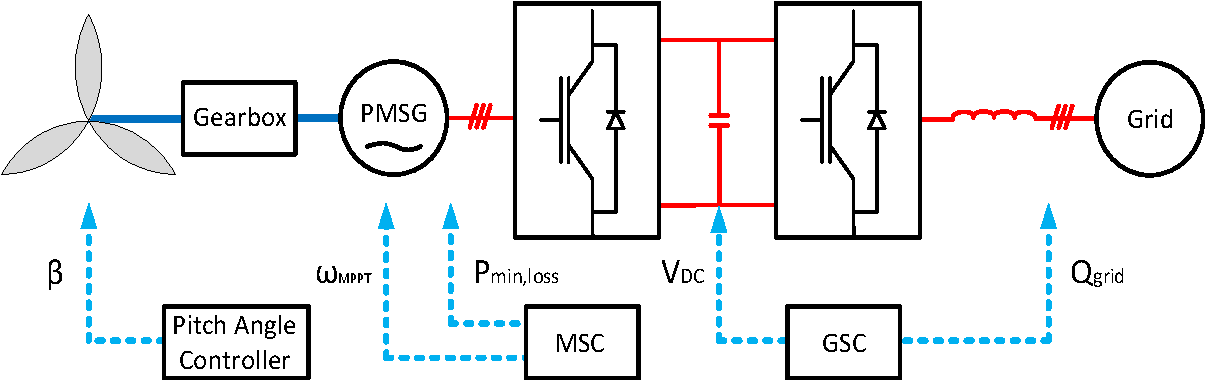
\includegraphics[width=1\linewidth]{windmodel2.png}
	\caption{Variable Speed Geared Wind Turbine Model}
	\label{varspeedpmsg}
\end{figure} 
Fig. \ref{varspeedpmsg} shows the modelling of variable speed PMSG wind turbine. The source of the power in these systems is the wind itself. The power is captured from the wind with the help of three-blade turbine. Three-blade turbine is the aerodynamic part of the system and it applies a aerodynamic torque to gearbox. In fact, this torque is the source of the movement and dictates the direction of the movement. Aerodynamic torque is applied to gearbox which establishes the connection between turbine and generator. In variable speed wind turbines, stator of the PMSG is not directly connected to grid. A back-to-back converter is used between generator and the electrical grid to ensure that the turbine speed is independent from the grid frequency. The converter which is connected to PMSG is called Machine Side Converter (MSC) meanwhile the one connected to grid is called Grid Side Converter(GSC). Moreover, GSC is connected to grid with a filter in order to filter out high frequency currents due to switching action. 
\subsection{Aerodynamic Model}
Aerodynamic model is the sub-model that captures power from the wind. The output of this block is the aerodynamic torque that rotates the turbine. However, the wind speed is not the only input. Turbine speed and pitch angle are also the inputs of the system since they affect the mechanical power that is captured from the wind.\par
The aerodynamic power of wind is given in Eq. (\ref{windpower}) where $\rho_{air}$ is air density in $kg/cm^{3}$, $R$ is the blade radius in $m$ abd $v_{WIND}$ is the wind speed in $m/s$. Note that this is the available power of the air that is striking the turbine swept area and it is not possible to extract that amount of energy. Otherwise, the air would be standstill behind the wind turbine \cite{Ackermann2005a}.
\begin{equation}
P_{WIND}=0.5\rho_{air}\pi R^{2} v_{WIND}^{3}
\label{windpower}
\end{equation}
The wind turbine captures a fraction of the available wind power that is denominated as power coefficient $C_{p}$. Therefore, turbine power captured from wind can be found with the Eq. (\ref{turbinepower}).
\begin{equation}
P_{TUR}=C_{P}P_{WIND}
\label{turbinepower}
\end{equation}
Power coefficient determines the amount of power and it is a non-linear function of the tip speed ratio, $\lambda$ and pitch angle, $\beta$. Tip speed ratio is a parameter proportional with turbine speed. It can be defined as the ratio of the speed in the turbine tip to the wind speed as in the Eq. (\ref{tipspeed}). Power coefficient for a specific tip speed ratio and pitch angle can be found with the Eq. (\ref{cp}) and (\ref{lambdai}) where $c_{1}$ is 0.5176, $c_{2}$ is 116, $c_{3}$ is 0.4, $c_{4}$ is 5, $c_{5}$ is 21 and $c_{6}$ is 0.0068 \cite{Heier}.\par
\begin{equation}
\lambda=\frac{\omega_{tur}R}{v_{WIND}}
\label{tipspeed}
\end{equation}
\begin{equation}
C_{p}(\lambda,\beta)=c_{1}(c_{2}/\lambda_{i}-c_{3}\beta-c_{4})e^{-c_{5}/\lambda{i}}+c_{6}\lambda
\label{cp}
\end{equation}
\begin{equation}
\frac{1}{\lambda_{i}}=\frac{1}{\lambda+0.08\beta}-\frac{0.035}{\beta^{3}+1} 
\label{lambdai}
\end{equation}
\begin{figure}[h!]
	\centering
	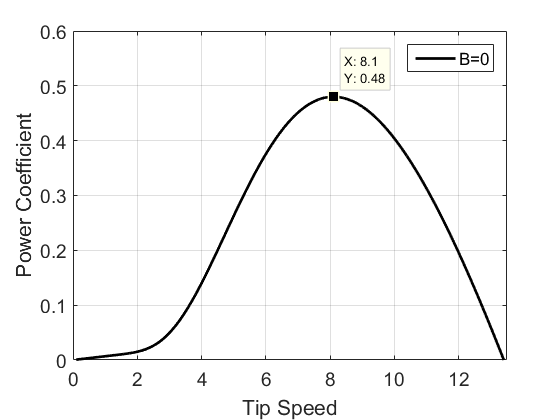
\includegraphics[width=.65\linewidth]{PowerCoefficient.png}
	\caption{Power Coefficient Variation with Tip Speed Ratio under Zero Pitch Angle}
	\label{variationofcp}
\end{figure} 
\par
Variation of power coefficient $C_{p}$ is given in Fig. \ref{variationofcp}. For the zero pitch angle, power coefficient has the maximum value of 0.48 for the tip speed ratio of 8.1. In order to ensure that the maximum of wind power is extracted, wind turbine should rotate a speed that gives the optimum tip speed ratio. 
\subsubsection{Pitch Angle Control}
According to Eq. (\ref{windpower}), wind power increases with the cube of the wind speed. Hence, wind power increases dramatically for the high wind speeds. In order to decrease power, pitch angle i.e. blade angle is increased. Since the power coefficient, $C_{p}$ is a function of the pitch angle, $\beta$, wind power can be curtailed with increased blade angle. Variation of power coefficient for two different pitch angle is shown in Fig. \ref{cpwithtwopitchangle}. Increasing pitch angle by $1.176^{\circ}$ decreases power coefficient by 10\%.\par
\begin{figure}[h!]
	\centering
	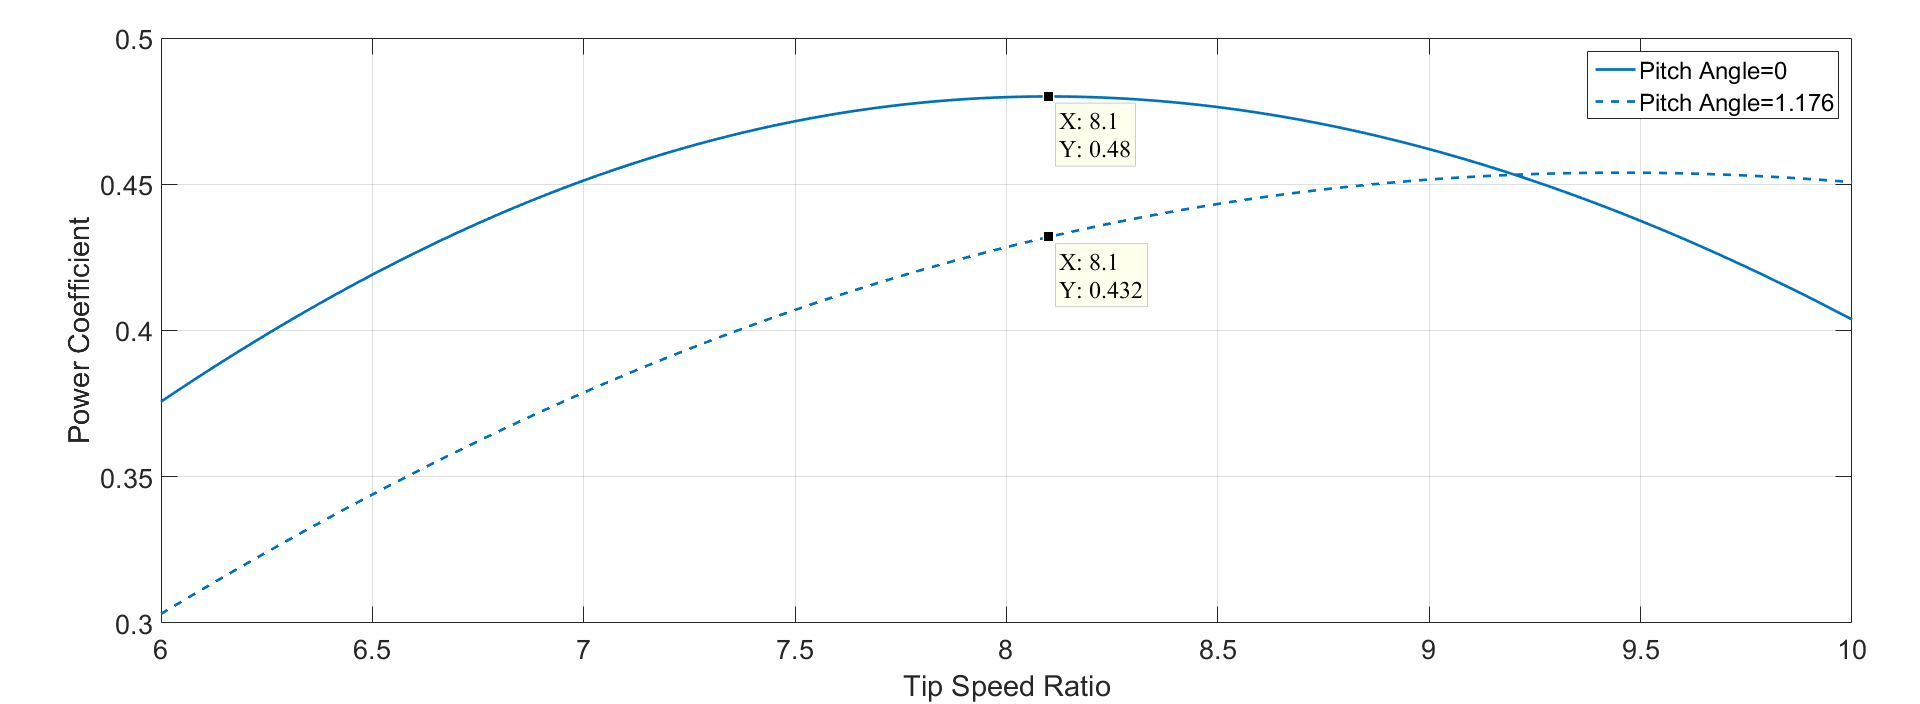
\includegraphics[width=.95\linewidth]{PowerCoefficient_with_varying_pitch.png}
	\caption{Power Coefficient Variation for Two Different Pitch Angle}
	\label{cpwithtwopitchangle}
\end{figure} 
As long as wind power is below the rated power, the wind turbine is operated in MPPT speed. This is ensured by obtaining optimal tip speed ratio. This means that for zero pitch angle, MPPT speed is increased linearly with wind speed. Before reaching rated power, MPPT speed might reach maximum generator speed. In this case, wind turbine reference speed will be the maximum generator speed. However, turbine speed cannot be decreased down to reference speed when the torque limit is reached. Hence, the pitch angle should be increased to regulate the turbine speed. Pitch angle controller is depicted in Fig. \ref{pitchcontroller}. Note that the pitch angle is increased when the speed exceeds maximum generator speed. Otherwise, the pitch angle kept as zero. 
\begin{figure}[h!]
	\centering
	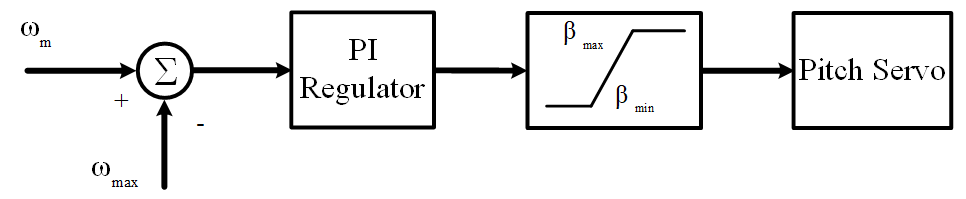
\includegraphics[width=.9\linewidth]{pitchcontroller.png}
	\caption{Pitch Angle Control Diagram}
	\label{pitchcontroller}
\end{figure}

\subsection{Gearbox}  
Variable speed PMSG wind turbines have a gearbox between turbine and generator except for direct-drive wind turbines. The gearbox increases angular speed and decreases the torque in the generator side.By decreasing the rated torque, generator size and cost can be reduced since the generator size is almost proportional to rated torque due to constant shear stress \cite{Polinder2013aa}. Moreover, turbine speed is increased to the allowable speed range of the generator which is generally much higher than that of wind turbines. Otherwise, generator should have high pole numbers. \par
A gearbox model is depicted in Fig. \ref{gearboxmodel}. They are mainly used for speed and torque conversion. It should be noted that the gearboxes are not full efficient systems. Therefore, the output torque of the gearbox would be lower than the ratio of input torque to gearbox conversion ratio. Direct-drive systems are based on the elimination of the gearbox systems by direct connection between turbine and generator in order to increase efficiency and reliability \cite{Chen2009b}. In this study, gearbox system is modelled with 100\% efficiency. 
\begin{figure}[h!]
	\centering
	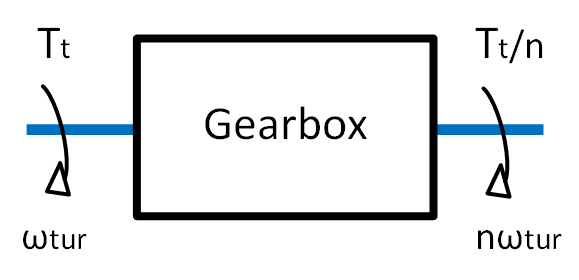
\includegraphics[width=.45\linewidth]{gearbox.png}
	\caption{Gearbox Modelling}
	\label{gearboxmodel}
\end{figure}

\subsection{Permanent Magnet Synchronous Generator}
\label{pmsgsection}
PMSGs are generally preferred over electrically excited synchronous generators due to high efficiency due to the fact that absence of electrical excitation on the rotor decreases losses. Besides, slip ring is not needed in the generator which also decrease the maintenance. Dynamical equations of the salient pole PMSG are projected on a reference frame which rotates synchronously with magnet flux and given in Eq. (\ref{v1d}) and (\ref{v1q}) where $R_{1}$ is stator resistance in $\Omega$, $L_{sd}$ and $L_{sq}$ are d and q axis inductances in $H$, $i_{ad}$ and $i_{aq}$ are d and q axis currents in $A$, $\omega$ is the electrical angular frequency in $rad/s$ $\psi_{f}$ is magnet flux linkage in $Vs$ \cite{Ackermann2005a}. 
\begin{equation}
v_{1d}=R_{1} i_{ad}+L_{sd}\frac{di_{ad}}{dt}-L_{sq}\omega i_{sq}
\label{v1d}
\end{equation}
\begin{equation}
v_{1q}=R_{1} i_{aq}+L_{sq}\frac{di_{aq}}{dt}+L_{sd}\omega i_{sd}+\omega \psi_{f}
\label{v1q}
\end{equation}
Another important PMSG parameter is the power in dq frame. The power expression is given in Eq. (\ref{pmsgpower}). The electromechanical torque can be found by the relation between power and angular speed. The torque expression is also given in Eq. (\ref{pmsgtorque}) where p is the number of pole pair.
\begin{equation}
P_{elm}=\frac{3}{2}\omega i_{aq} (\psi_{f}+i_{ad}(L_{sq}-L_{sd}))
\label{pmsgpower}
\end{equation}
\begin{equation}
T_{e}=\frac{P_{elm}}{w_{m}}=\frac{P_{elm}}{w/p}=\frac{3}{2}p i_{aq} (\psi_{f}+i_{ad}(L_{sq}-L_{sd}))
\label{pmsgtorque}
\end{equation}

Given equations are defined for salient pole machines. If the clyndrical rotor machine is used, the torque equation reduces to the Equation \ref{pmsgtorque2}.
\begin{equation}
T_{e}=\frac{3}{2}p i_{aq} \psi_{f}
\label{pmsgtorque2}
\end{equation}

\subsection{Machine Side Converter}
Variable speed wind turbines are equipped with the Back-to-Back converters in order to decouple grid frequency and the turbine speed. This gives wind turbine degree of freedom for the rotational speed. In this way, turbine is able to capture the maximum available power from wind. Machine Side Converter (MSC) i.e. Generator Side Converter is the converter that is connected between generator and DC-bus. The three phase generator output AC voltage is converted to DC voltage.
Conversion from AC to DC can be achieved by three-arm full bridge converters. This converter can be equipped with uncontrolled, semi-controlled and fully-controlled switches. Fully-controlled switches such as MOSFET,IGBT are commonly used in the industry and gives two control parameters to the user. \par
Voltages and currents are generally transformed into synchronously rotating reference frame or also called dq frame. Since the frame is rotating in synchronous speed, three-phase phasors are transformed to DC quantities. Therefore, its control becomes easier \cite{Kazmierkowski2002}. Proportional-integral (PI) controllers are associated with the dq control structure due to their satisfactory behaviour interaction to DC variables \cite{Blaabjerg2006a}. Hence, the control in the back-to-back converter is achieved with PI controllers in the dq frame. \par
\begin{figure}[h!]
	\centering
	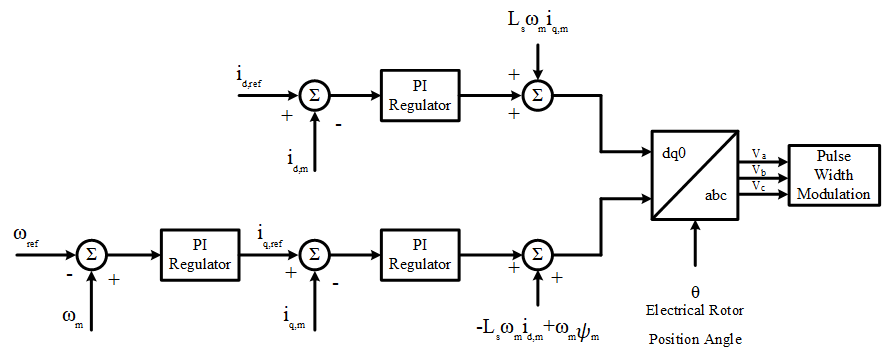
\includegraphics[width=.95\linewidth]{msc.png}
	\caption{Machine Side Control Diagram}
	\label{msc}
\end{figure}
The control diagram of the MSC is depicted in Fig. \ref{msc} according to the study in \cite{Chinchilla2006}. In dq frame, it is possible to control two parameters. One of these parameters is the d-axis current. It can be set zero in order to decrease the stator copper losses. The other parameter is the q-axis current that is proportional to the electromagnetic torque as it can be observed in the Eq. (\ref{pmsgtorque2}). However, q-axis current or torque is controlled in order to regulate the turbine speed. Therefore, turbine speed is adjusted such that the turbine will capture maximum available power in the wind. 
\subsection{Grid Side Converter}
Grid Side Converter (GSC) or Line Side Converter (LSC) is the converter that is connected between DC-link capacitance and grid. GSC works as an inverter that injects current synchronous with grid voltage. Currents and voltages are transformed into synchronously rotating frame that is aligned with the grid voltage. Therefore, d-axis current determines the amount of current which is in phase with the grid voltage meanwhile q-axis current determines amount of current that is out of phase with the grid voltage. In other words, injecting d-axis current injects active power to grid meantime q-axis current injects reactive power to grid. \par
The responsibility of the GSC is regulating DC voltage and the reactive power injected to grid. The control diagram of the GSC is given in Fig. \ref{gsc}. As seen from the figure, DC-bus voltage is regulated by controlling the d axis current. If the DC-bus voltage increases above the reference value, d-axis current reference is increased. As a result, active power increases. Increased active power also decreases the DC-bus voltage level. Reference value of the q-axis current is set to zero in normal operation, consequently unity power factor. For Low Voltage Ride-Through studies, q-axis current is determined according to the reactive power value requirement. \cite{Orowska-Kowalska2014} \par
\begin{figure}[h!]
	\centering
	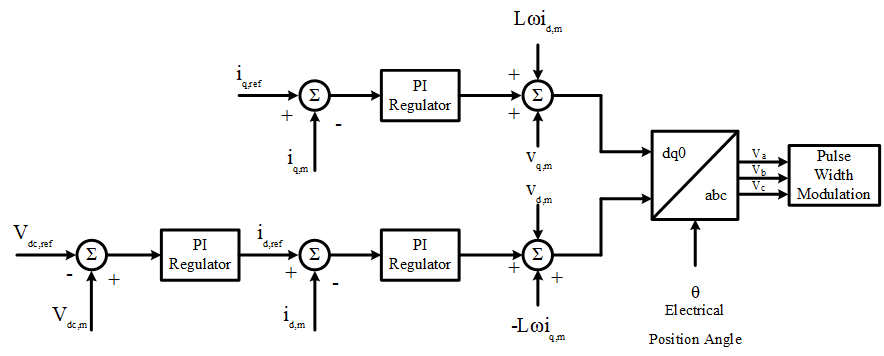
\includegraphics[width=.98\linewidth]{gsc.png}
	\caption{Grid Side Control Diagram}
	\label{gsc}
\end{figure}
GSC is connected to grid through an filter. Therefore, the output voltage of the converter is not equal to the that of grid. The relation between converter voltage, grid voltage and current is derived through Eq. (\ref{crossilk}) to (\ref{crosscomp2}) where $v_{c}$ is the converter voltage, $v_{g}$ is the grid voltage and  $i_{g}$ is the grid current measured in the grid side. As it is observed in Eq (\ref{crosscomp1}) and (\ref{crosscomp2}), converter side voltage includes same axis grid voltage and a term proportional to cross axis current which is called cross-coupled term. Therefore, the outputs of the inner PI regulators are compensated and forwarded to Pulse Width Modulation after transformation to three-phase voltages.
\begin{equation}
\overline{v_{c}}=v_{dc}+jv_{qc}
\label{crossilk}
\end{equation}
\begin{equation}
\overline{v_{g}}=v_{dg}+jv_{qg}
\end{equation}
\begin{equation}
\overline{i_{g}}=i_{dg}+ji_{qg}
\end{equation}
\begin{equation}
\overline{v_{c}}=\overline{v_{g}}+\overline{i_{g}}j\omega L
\end{equation}
\begin{equation}
v_{dc}+jv_{qc}=v_{dg}+jv_{qg}+j\omega L (i_{dg}+ji_{qg})
\end{equation}
\begin{equation}
v_{dc}=v_{dg}-\omega L i_{qg}
\label{crosscomp1}
\end{equation}
\begin{equation}
v_{qc}=v_{qg}+\omega L i_{dg}
\label{crosscomp2}
\end{equation}
\section{Synthetic Inertia Implementation}
As explained in Chapter \ref{chp:2} Section \ref{swing}, synchronous generators changes its speed according to the balance between input mechanical and electromechanical powers. The inverse case is also true. In other words, if the frequency changes, the electromechanical power of the generators also change. Synthetic inertia is the method that implements this behaviour on the renew able energy systems. It is possible to change the active power output of the wind turbines if these are connected to grid with full scale power electronics. The increase in the active power should be proportional to change of frequency and the inertia of the renewable energy system. Even though renewable energy system does not have inertia, inertial support with desired inertia constant can be implemented in the system as long as a stored energy exists in the system.\\
In order to implement synthetic inertia in the system, a relation between frequency and active power of the wind turbine should be constructed. Wind turbine in this study is variable speed wind turbine with full scale power electronics. The speed of the turbine is controlled by MSC such that active power is adjusted.Inertial support modification is depicted in Fig. \ref{modifiedmsc}. The new value of the active power is determined according to the swing equation. However, the wind turbine in this study is operated with a reference speed rather than a reference power. Therefore, the assigned power value should be used in order to yield the q-axis current reference value. Reference q-axis current is derived between the Eq. (\ref{inertialsupport1}) to Eq. (\ref{inertialsupport4}).
\begin{figure}[h!]
	\centering
	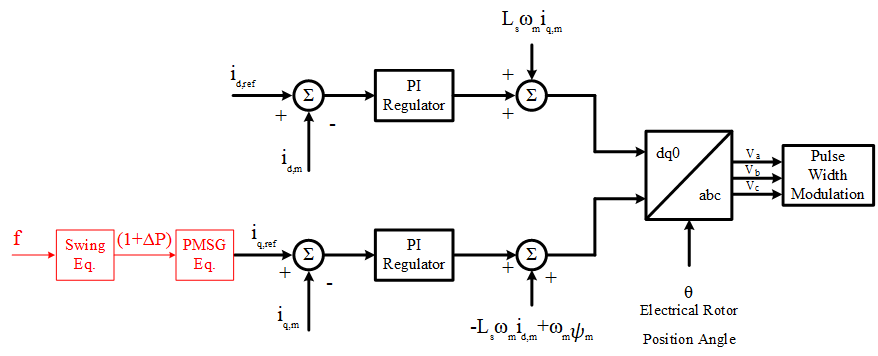
\includegraphics[width=.98\linewidth]{msc_modified.png}
	\caption{Modified MSC for Inertial Support}
	\label{modifiedmsc}
\end{figure}
\begin{equation}
P_{new}=(1+\Delta P) P_{pre}
\label{inertialsupport1}
\end{equation}
\begin{equation}
T_{new} \omega_{m}=(1+\Delta P) T_{pre} \omega_{pre}
\label{inertialsupport2}
\end{equation}
\begin{equation}
\frac{3}{2} p \psi_{f} i_{q,new} \omega_{m}=(1+\Delta P) \frac{3}{2} p \psi_{f} i_{q,pre} \omega_{pre}
\label{inertialsupport3}
\end{equation}
\begin{equation}
 i_{q,ref}=i_{q,new}=(1+\Delta P) \frac{i_{q,pre} \omega_{pre}}{ \omega_{m}} 
\label{inertialsupport4}
\end{equation}

\subsection{Synthetic Inertia Activation Schemes}
Another issue about inertial support is the time instant to trigger synthetic inertia. In the literature, continuous operation, under-frequency trigger and maximum-frequency gradient are discussed \cite{Gonzalez-longatt2015}. It is obvious that continuous operation would create oscillations in active power output due to the continuous deviations in grid frequency. This is an unrealistic operation and is used for comparison purposes.\par
Second activation method is the under-frequency trigger which is the activation when the frequency decreases below a threshold value. It can be used for capturing the time instant for the inertial support. However, power grid might be in a stable point even if the frequency is 49.8Hz. Therefore, this method would be unsuccessful depending on the disturbance event. \par 
Third activation scheme is the maximum-frequency gradient trigger. It uses a controller that is very similar to RoCoF relays and tracks the frequency gradient. Once the frequency gradient is below a threshold value, the synthetic inertia is activated. Since the severity of frequency disturbance event is related to the RoCoF, this activation scheme is the most remarkable scheme \cite{Gonzalez-longatt2015}. In this study, maximum-frequency gradient is used with a threshold value of 0.1Hz/s. 
\subsection{Source of the Inertial Support}
Renewable energy systems convert the energy captured from wind or sun to the electrical energy. Hence, the renewable energy systems cannot determine the amount of power in contrast the conventional systems. A thermal power plant, for instance, adjusts its power output as desired. However, the source of power in renewable energy is constant for a definite wind speed or solar radiation. This is why a spare energy is required in order to change the power output. \par
Energy stored in DC bus capacitance is the only stored energy in PV systems. The amount of energy is given in Eq. (\ref{electrostatic}) and negligible for inertial support studies. In the wind energy systems, there exists huge amount of kinetic energy in wind turbine generator and blades in addition to electrostatic energy. The kinetic energy expression is given in Eq. (\ref{kineticenergy}). Note that $J_{total}$ is the equivalent inertia in the generator side and $\omega_{m}$ is the speed of the generator.
\begin{equation}
E_{electrostatic}=\frac{1}{2} C_{DC}V_{DC}^{2}
\label{electrostatic}
\end{equation}
\begin{equation}
E_{kinetic}=\frac{1}{2} J_{total}\omega_{m}^{2}
\label{kineticenergy}
\end{equation}
Note that the amount of kinetic energy is dependent on the generator speed. Therefore, the stored energy in wind turbines changes according to the generator speed. Moreover, it can also be concluded that the energy is dependent on the wind speed. However, the generator speed is kept constant if the wind speed increases above the rated wind speed. \par
To illustrate the situation better, the electrostatic energy stored in DC bus and kinetic energy in turbine equivalent inertia are compared for GE2.75-103 wind turbine. The wind turbine has a DC bus capacitance of $27mF$ and $1200V$ DC link voltage. The corresponding electrostatic energy is calculated in Eq. (\ref{electrostatic2}). The generator speed of the corresponding generator is between $550rpm$ and $1735rpm$. The total turbine inertia is $1058.2 kgm^2$ in generator side. The minimum and maximum kinetic energy values are calculated in Eq. (\ref{kineticenergymin}) and (\ref{kineticenergymax}). These values are found out to be 90 and 900 times of the electrostatic energy stored in DC bus capacitance.
\begin{equation}
E_{DC-Link}=\frac{1}{2} 27 (10^{-3}) 1200^{2}=19.44kJ
\label{electrostatic2}
\end{equation}
\begin{equation}
E_{kinetic,min}=\frac{1}{2} (1058.2) 57.6^{2}=1755.17kJ
\label{kineticenergymin}
\end{equation}
\begin{equation}
E_{kinetic,max}=\frac{1}{2} (1058.2) 181.7^{2}=17466.02kJ
\label{kineticenergymax}
\end{equation}